\section{tasks::findinterlacedord Class Reference}
\label{classtasks_1_1findinterlacedord}\index{tasks::findinterlacedord@{tasks::findinterlacedord}}
Inheritance diagram for tasks::findinterlacedord::\begin{figure}[H]
\begin{center}
\leavevmode
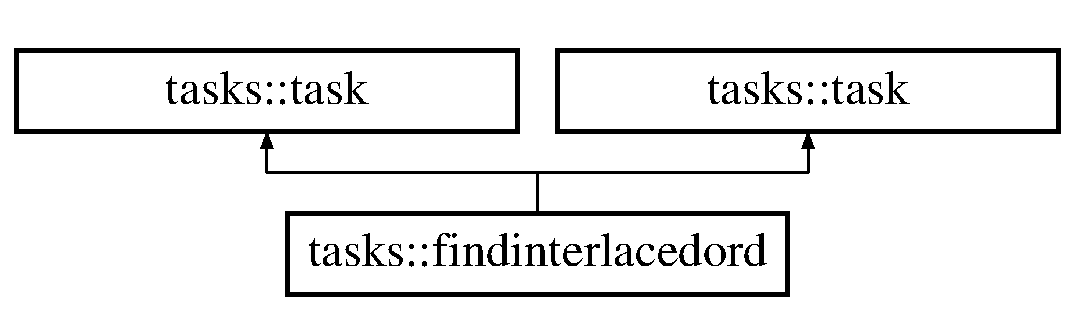
\includegraphics[height=2cm]{classtasks_1_1findinterlacedord}
\end{center}
\end{figure}
\subsection*{Public Member Functions}
\begin{CompactItemize}
\item 
def \textbf{run}\label{classtasks_1_1findinterlacedord_28bad17fea4f445072777c823ac9fc5b}

\item 
def \textbf{run}\label{classtasks_1_1findinterlacedord_28bad17fea4f445072777c823ac9fc5b}

\end{CompactItemize}
\subsection*{Static Public Attributes}
\begin{CompactItemize}
\item 
string \textbf{name} = '{\bffindinterlacedord}'\label{classtasks_1_1findinterlacedord_6ae93f890694bbeec91ab0dfc91108a8}

\item 
string \textbf{button\-Text} = 'Find interlaced order locs.'\label{classtasks_1_1findinterlacedord_e33974a031452ec69f27e4cf484a5d47}

\item 
int \textbf{inthread} = 0\label{classtasks_1_1findinterlacedord_559c35c33bc9aa414e9a9ef08a2e1a68}

\end{CompactItemize}


\subsection{Detailed Description}


\footnotesize\begin{verbatim}Interactively define and trace the location of interlaced spectral orders
   using a well-exposed order-definition frame. 
\end{verbatim}
\normalsize
 



The documentation for this class was generated from the following files:\begin{CompactItemize}
\item 
old/PANICtool-1.0/tasks.py\item 
old/tasks.py\end{CompactItemize}
